\section{Qu’est-ce qu’un graph distribué}
Pour comprendre ce qu’un graph distribué, il faut d’abord qu’est-ce que un système distribuée, par-ce-que un graphe distribuée n’est que un cas particulier des systèmes distribuées.\\
Un système distribué [b.11], également connu sous le nom de "calcul distribué", est un système comportant de multiples composants situés sur différentes machines qui communiquent et coordonnent des actions afin d'apparaître comme un seul système cohérent pour l'utilisateur final.\\
Un système distribué, au contraire d’un système centralisé, son état a un moment t est stocké dans plusieurs machines, c’est-à-dire que pour savoir l’état du système à un certain moment il faut savoir l’état des tous les machines que le compose. Ces caractéristiques introduisissent plusieurs avantages ainsi que des inconvénients :\\

\textbf{Les avantages :}
\begin{itemize}[label=\textbullet]
\item  Scalabilité horizontale : Comme le calcul se fait indépendamment sur chaque nœud, il est facile et généralement peu coûteux d'ajouter des nœuds et des fonctionnalités supplémentaires si nécessaire.\\
\item  Fiabilité : la plupart des systèmes distribués sont tolérants aux pannes car ils peuvent être constitués de centaines de nœuds qui fonctionnent ensemble. Le système ne subit généralement pas de perturbations si un nombre de machines tombe en panne généralement le système distribué qu’utilise des algorithmes de consensus robustes tel que RAFT [b.10] ou PAXOS, peuvent se permettre jusqu’à N / 2 machines en panne si le nombre des machines est N + 1.
\item  Performance : Les systèmes distribués sont extrêmement efficaces car les charges de travail peuvent être fragmentées et envoyées à plusieurs machines. Sauf que la tâche difficile dans la plupart des systèmes consiste à comment le fragmenter, de manière à ce que l’avantage obtenu dépasse les désavantages, ceci reste encore un sujet de recherche intense.
\end{itemize}

\textbf{Les désavantages :}
\begin{itemize}[label=\textbullet]
\item  Ordonnancement : Un système distribué doit décider quelles tâches doivent être exécutées, quand et où elles doivent être exécutées. Les ordonnanceurs ont finalement des limites, ce qui entraîne une sous-utilisation du matériel et des durées d'exécution imprévisibles.
\item  Latence : Plus votre système est largement distribué, plus vous pouvez connaître une latence dans les communications. Cela conduit souvent les équipes à faire des compromis entre disponibilité, cohérence et latence.
\item  Observabilité : La collecte, le traitement, la présentation et le suivi des mesures d'utilisation du matériel pour les grands clusters constituent un défi important.
\end{itemize}

Dans le même contexte les systèmes distribuées peuvent se manifester sous forme de plusieurs architectures voici deux :\\
\begin{itemize}[label=\textbullet]
\item  Peer-to-peer : Il n'y a pas de machines supplémentaires utilisées pour fournir des services ou gérer des ressources. Les responsabilités sont uniformément réparties entre les machines du système, appelées "pairs", qui peuvent servir soit de client, soit de serveur. BitTorrent est l’un des exemples les plus connues car chaque machine que l’installe devient fournisseur de service pour les autres utilisateurs.
\item  Les clusters : sont des systèmes distribués fabriqués à partir de composants de commodité (ordinateur personnel, serveur, Raspberry PI …etc.). Les nœuds sont des machines contenant un ou quelques processeurs, de la mémoire RAM et souvent du stockage sur disque.
Les nœuds sont reliés par une interconnexion de produits, qui est disponible en plusieurs formes, notamment Gigabit Ethernet et Infiniband. En utilisant de composants de commodité, les clusters ont un rapport prix/performance exceptionnel par rapport à la plupart des autres formes d'informatique haut de gamme.
PGX Distribuée en mode développement tire profit de cette architecture, car elle offre la meilleure performance due à la petite latence qui génère parce que les machines sont interconnectées directement.
\item  ...
\end{itemize}

Maintenant qu’on a compris ce que un système distribuée, et que un graph distribuée et l’un des systèmes il faut décrire les spécificités de ce type des graphes, ces avantages et ces inconvénients.

\begin{figure}[h!]  
  \centering
    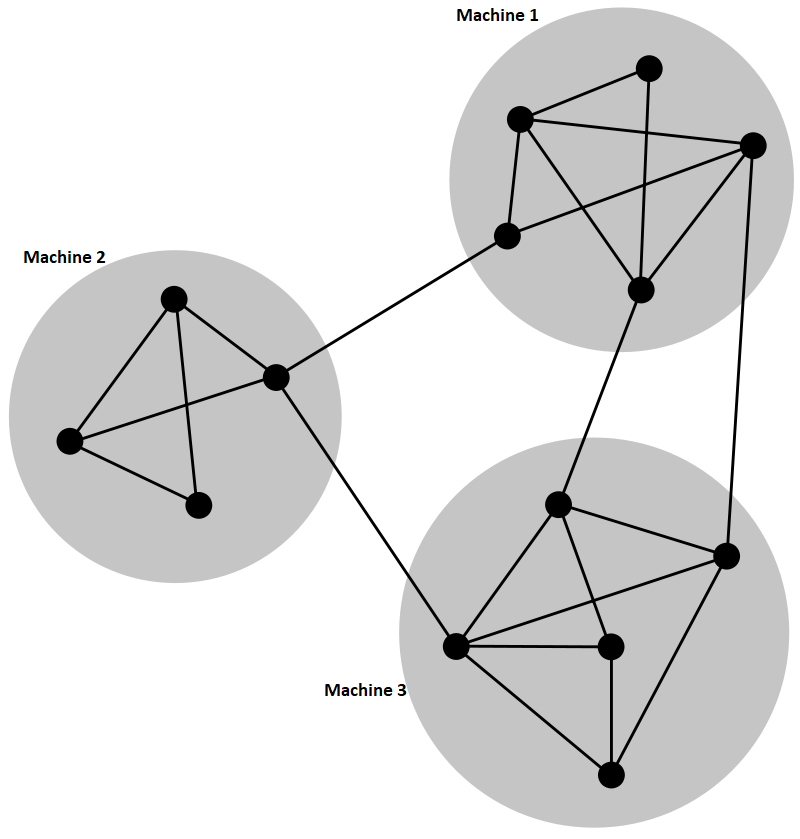
\includegraphics[width=1\textwidth]{chapitre2/Figures/Network_Community_Structure.svg.png}
  \caption{Exemple d'un graphe distribué sur trois machines}
\end{figure}

Si on observe bien on peut remarquer que les graphes sont partout dans notre entourage, le plus simple exemple sont les routes qui interconnecte les villes, les villes seront modélisées en sommets et les routes comme les arêtes et à partir de cette modélisation en peut extraire un grand nombre d’informations grâce aux outils développes par la théorie des graphes. L’algorithme de Dijkstra étant un exemple d’algorithme que donc le cas idéal (Le graphe est statique, pas d’embouteillages, vitesse fixe …etc.), permet d’extraire le chemin le plus court entre deux villes en un temps polynomial. Dans le cas ou le graphe et petite en peut implémenter, ce algorithme pour s’exécuter sur une seule machine et on auras le résultat prévue, mais lorsque le graphe ne peut pas être chargé sur une seule machine il faut opter pour un graphe distribuée.\\
Implémenter un graphe distribué n’est pas une tâche simple, la plus grande problématique consiste à le partitionner en des sous-graphes faiblement couplé pour diminuer ainsi la communication entre les machines qui est souvent la source de plus grande perte de performance. Il existe plusieurs méthodes et techniques pour partitionner un graphe, tous ce concentre sur le fait de démineur les connexion entre les sous-graphes dans chaque machine et en même temps d’assurer que la charge est balancé c’est-à dire que la différence entre le nombre des sommets et arrêts dans chaque nœud est petite.\\
Parmi les techniques les plus utilisée en trouve DFS ou BFS pour trouver toutes les composantes faiblement et fortement connectées, et l’utilisation des sommets fantôme (Ghost nodes/vertices) pour le sommet qui sont partagées entre les machines. Ces calcules préalables ainsi génère des coûts indirects, ce qui rend le chargement du graphe en sa forme final qui peut être exploité par l’utilisateur plus lente, en verra dans le chapitre du benchmarking avec TPC-H, comment j’ai souffert avec ce problème et comment j’ai pu réduire ce temps significativement spécifiquement pour la tâche que j’avais en main.\\
